\section{SimCLR}


\begin{frame}[fragile]{SimCLR}
    \begin{columns}
    \begin{column}{0.7\textwidth}
        \begin{itemize}
            \item Goal: 用 contrastive learning 方法学习图片的 visual representations。
            \item 训练集是若干无标签图像,希望对每个图像输出一个 feature vector。
        \end{itemize}
        右图中,$f$ 是一个神经网络,输入扰动后的图像,输出一个 feature vector。$g$ 是一个 projection head,将 feature vector 投影到一个用于衡量相似度的空间。
        
        $T$ 是对图像施加各种可能扰动的集合,例如随机裁剪、旋转、噪声、模糊等。
    \end{column}
    \begin{column}{0.3\textwidth}
        \begin{center}
            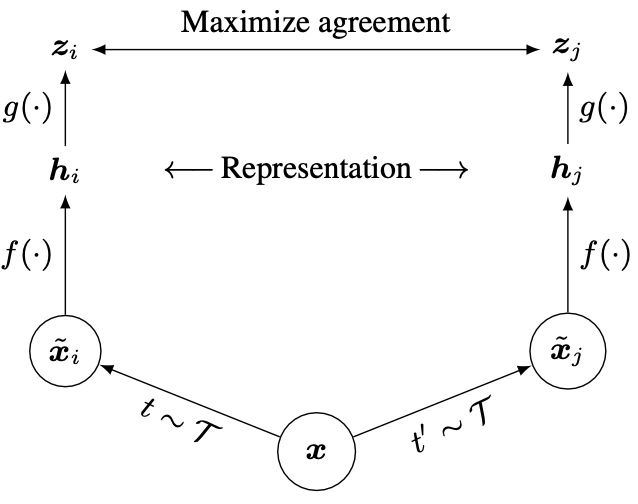
\includegraphics[width=\textwidth]{assets/simclr.png}
        \end{center}
    \end{column}
    \end{columns}
\end{frame}

\begin{frame}{SimCLR Algorithm}
    \begin{columns}
        \begin{column}{0.65\textwidth}
            \begin{itemize}
                \item Note: 其中 $\ell(i, j)$被称为 InfoNCE loss。
            \end{itemize}
        \end{column}
        \begin{column}{0.37\textwidth}
            算法:
            \begin{center}
                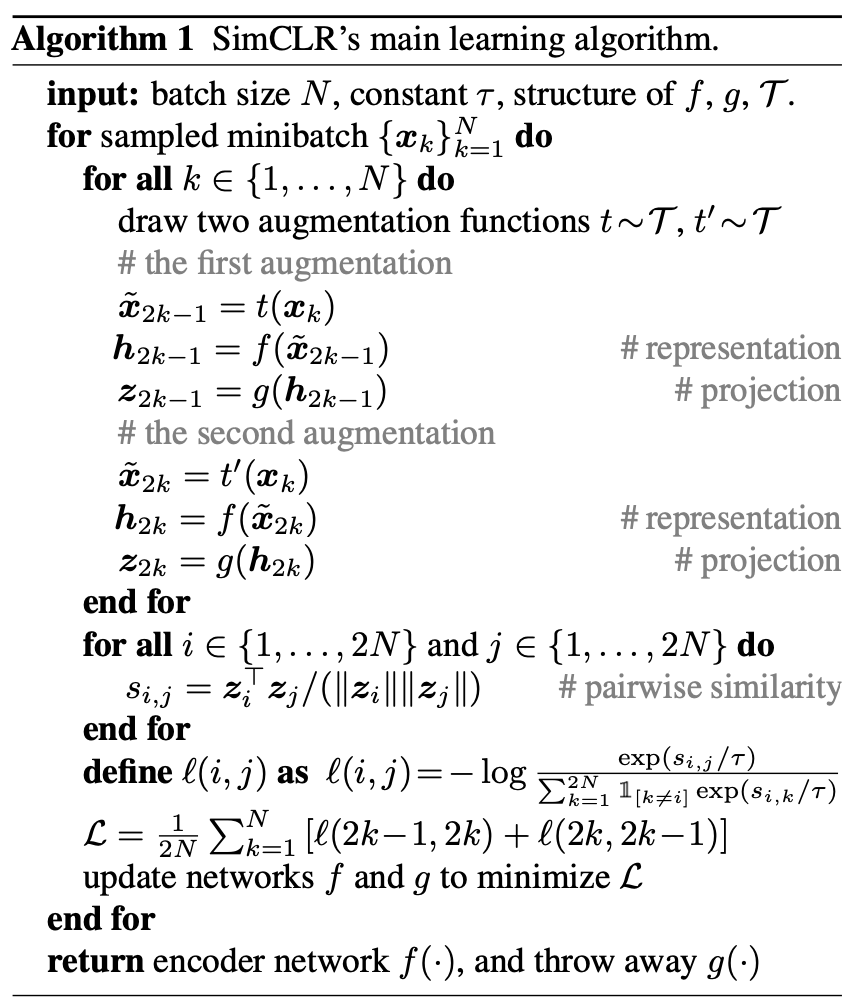
\includegraphics[width=\textwidth]{assets/simclra.png}
            \end{center}
                \end{column}
        \end{columns}
    
\end{frame}

\begin{frame}{Contrastive Learning is spectral clustering on similarity graph}
    Yang Yuan 组的一篇论文指出:
    \begin{itemize}
        \item 定义 Cross entropy loss $H_\pi^{k}(Z) = \mathbb{E}_{W_X\sim P(\cdot; \pi)} \left[ \log P(W_Z = W_X; K_Z) \right]$。
        \item 可以证明:Cross entropy loss 等价于 InfoNCE loss;
        \item Cross entropy loss 隐式在 similarity graph 上执行了 spectral clustering
        \item 所以 SimCLR 可以看作是 spectral clustering on similarity graph。
    \end{itemize}
    (把他课件上的内容差不多记住,作业那道题会做应该就行了)
\end{frame}

\begin{frame}{CLIP}
    \begin{itemize}
        \item CLIP 是一种多模态学习方法,可以同时处理图片和文本。
        \item 细节:给定一个batch of image-text pairs $(image, text)$数据,CLIP用一个 image encoder 和一个 text encoder 分别将 image 和 text 转换为 feature vectors对,然后用 InfoNCE 作为loss function 训练 encoder。
        \item CLIP 也隐式执行了 spectral clustering。
    \end{itemize}
\end{frame}
